%%PACCHETTI
\documentclass[]{article}
\usepackage{amsmath}
\usepackage{wrapfig}
\usepackage[normalem]{ulem}
\usepackage{soul}
\usepackage{graphicx} % Required for inserting images
%\usepackage[left=2cm, right=2cm, top=2.5cm, bottom=2.5cm]{geometry}
\usepackage{circuitikz}
\usepackage{tikz}
\usepackage{pgfplots}
\usepackage{geometry}
\usepackage{makeidx}
\usetikzlibrary{positioning, fit}
\usetikzlibrary{positioning}
\usepackage{tocloft}
\usepackage{subcaption}
\usepackage{graphicx}
\usepackage{tcolorbox}
\usepackage{verbatim}
\usepackage{fancyhdr}
\usepackage{multirow}
\usepackage{cancel}
\usepackage{fontawesome}
\usepackage{adjustbox}
\usepackage[colorlinks=true, linkcolor=black, urlcolor=blue]{hyperref}
\pgfplotsset{compat=1.18}
\usepackage{nopageno}
\usepackage{booktabs}
\usepackage{float}
%Grafica del foglio
\geometry{a4paper, margin=2.0cm}
\usetikzlibrary{math}
\author{Alessandro Briccoli }
\graphicspath{ {./image/} } 
\pagestyle{fancy}

% Personalizzazione del piè di pagina
%\fancyfoot[L]{AB81}  % Sigla in basso a sinistra
\fancyfoot[C]{\thepage}  % Numero della pagina in basso al centro
\fancyfoot[R]{}  % Vuoto in basso a destra

\fancyhead[L]{} %vuoto in alto sx
\fancyhead[R]{\leftmark} %in alto a dx metto la sextion in cui siamo -> \leftmark 

% Rimuove le linee dell'intestazione e del piè di pagina predefinite
\renewcommand{\headrulewidth}{0pt}
\renewcommand{\footrulewidth}{0pt}

%definzione di comandi personalizzati
\newcommand{\brikbox}[1]{ %box per esempi
	
	
	\begin{tcolorbox}[
		left=5mm,
		right=5mm,
		colframe=black,
		colback=white,
		boxrule=0.5mm,
		sharp corners,
		width=\textwidth
		]
		#1 % Contenuto del tcolorbox passato come argomento
	\end{tcolorbox}
	%end_of_box
}

\newcommand{\numeratebrik}[1]{%elenco numerico
	\begin{enumerate}
		#1
	\end{enumerate}
	
}

\newcommand{\listbrik}[1]{%elenco puntato
	\begin{itemize}
		#1
	\end{itemize}
	
}

\newcommand{\img}[2]{ %inserire le immagini dentro box senza caption
	
	
	\begin{center}		
		\includegraphics[width=#1\linewidth]{image/#2}
	\end{center}
	
}

\newcommand{\imgcaption}[3]{ %inserire immagini con caption 
	\begin{figure}[h]
		\centering
		\includegraphics[width=#1\linewidth]{image/#2}
		\caption{#3}
		\label{fig:#2}
	\end{figure}
}


\newcommand{\systemine}[1]{
	\[
	\begin{cases}
		#1
	\end{cases}
	\]
}


\begin{document}
	\thispagestyle{empty}
	\begin{figure}[h] %logo muner
		\centering
		
\includegraphics[height=4cm, width=10cm]{img/Muner_Color} 
	\end{figure}
	
	\begin{center}  %titolo 
		\hspace{2em}
		\\
		{\LARGE\textbf{Automotive Technologies for Ranging, Vision and Connectivity}}
		\hspace{2em}
	\end{center}
	
	\thispagestyle{empty}
	\vspace*{\fill} 
	\begin{center}
		{\LARGE\textbf{LAB REPORT ON A PATCH ANTENNA}}
	\end{center}
	\vspace*{\fill}
	
	\vspace{1cm} 
	\vspace{1cm} 
	\begin{flushleft}
		Authors:\\
		\hspace{1.5em}Alessandro Briccoli, alessandro.briccoli@studenti.unipr.it\\
		\hspace{1.5em}Luca Dall'Aglio, luca.dallaglio2@studenti.unipr.it
		
	\end{flushleft}
	
	\vspace{2cm} 
	\begin{center}
		Academic Year 2024/2025
	\end{center}
	
	\newpage
	
	\thispagestyle{empty}
	\tableofcontents
	
	\newpage
	\setcounter{page}{1}
	\subsection*{GROUP 1}
	\textit{Design a patch antenna working (SWR $<$ 2) at the frequency of 2.6 GHz with a tolerance of $\pm 2.5\%$. The substrate is FR4 with $\varepsilon_r = 4.1 \cdot (3/f[\text{GHz}])^{0.025}$, $\tan(\delta) = 0.025$, and thickness $h = 1.6$ mm. The metal is copper with $t = 35$ $\mu$m thickness. The antenna must be centered on top of a square ground plane with side length equal to $c / (f\sqrt{\varepsilon_r})$ and must be fed by a microstrip transmission line connected to an edge-mount $50 \, \Omega$ connector.}
	\section{SUMMARY}
	The objective of this report is to present a detailed account of the laboratory experience with patch antennas. The document thoroughly outlines all the stages of the patch antenna design process, beginning with the theoretical framework, followed by the design phase, and concluding with the experimental analysis. Furthermore, it includes a comparison between the simulation results and the real-world measurements obtained during testing.
	\section{INTRODUCTION}
	The objective of the laboratory experiment was to design a patch antenna with a resonant frequency of 2.6 GHz, as specified in the group specifications. A patch antenna, also referred to as a microstrip antenna, is a relatively straightforward type of antenna that offers numerous advantages, including its lightweight, cost-effectiveness, and simple integration with accompanying electronic components.\\
	Developed in the early 1970s for spatial and aeronautics applications, this antenna gained popularity thanks to its lightweight and low volume, low fabrication cost due to mass production with PCB techniques, easy integration with printed circuits, and conformability. It is also suitable for mobile wireless applications.\\
	However, it should be noted that this antenna type possesses a comparatively larger size in comparison to alternative antenna designs. For instance, some patch antennas are approximately half a wavelength on each side. Additionally, there are some disadvantages, such as low efficiency, narrow bandwidth, low gain, and poor polarization purity.\\
	The architecture of a patch antenna is very simple: it consists of a ground plane, a dielectric material substrate, and a patch of metal. During the laboratory lectures, firstly the patch antenna was designed by using CST Studio. To do this, the first task was to retrieve, from the theory lectures, the method to compute the main parameters of a microstrip antenna. Subsequently, the design of the antenna block was initiated, followed by the execution of simulations to assess its performance. The utilization of CST Studio enabled the exploration of various parameters, facilitating the optimization of the antenna's configuration. The final laboratory lecture focused on the collection of measurements from the fabricated antenna, thereby enabling the comparison of the simulation outcomes with real-world observations.
	\newpage
	\section{THEORY} 
	\subsection{Patch antenna dimensions}
	In order to design a patch antenna, it is first necessary to define the different formulas used to derive antenna dimensions from a theoretical point of view.\\
	A patch antenna, as we can see in the figure below, shares similarities with a microstrip transmission line, but there is a crucial distinction between the two. The patch antenna is designed to radiate, and consists of a metal patch that is placed on top of a dielectric substrate, which is then positioned on a metallic ground layer. The purpose of the substrate is to block radiation beyond it, thereby ensuring that the radiation is supplied exclusively in the positive axis, which, in this case, is the Z axis.\\
	\begin{figure}[h]
		\centering
		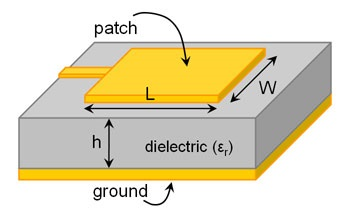
\includegraphics[width=0.4\linewidth]{img/img1}
		\caption{Structure of a Patch Antenna}
		\label{fig:img1}
	\end{figure}
	
	As mentioned above, we can see the patch antenna as a microstrip line of length $L_p$ and width $W_p$, in particular: 
	\begin{equation}
		L_p=m\frac{\lambda}{2}
	\end{equation} 
	and 
	\begin{equation}
		W_p=\frac{c}{2f_r}\sqrt{\frac{2}{\varepsilon_r+1}}
		\label{Wp}
	\end{equation}
	where: 
	\begin{itemize}
		\item $\lambda$ is the wavelength 
		\item $c=3 \cdot 10^8 m/s$ is the speed of light
		\item $f_r$ is the resonance frequency of the antenna
		\item $\varepsilon_r$ is the dielectric constant of the substrate material, in our case is FR4
		
	\end{itemize}
	\subsection{Fringing effect} 
	The resonance condition for a patch antenna is typically given by \( L = \frac{\lambda}{2} \). However, as we can see in the figure below, due to edge effects, the actual path length is slightly longer, with a variation \( \Delta L \).
	\begin{figure}[h]
		\centering
		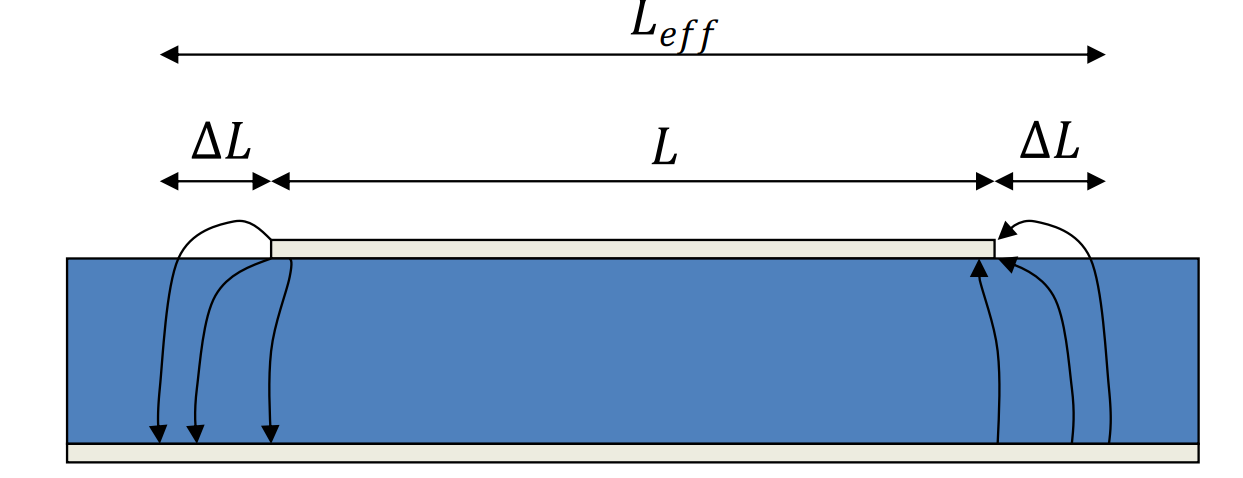
\includegraphics[width=0.4\linewidth]{img/img2}
		\caption{The electric field lines curve at the edges, increasing the electric length of the patch.}
		\label{fig:img2}
	\end{figure}
	
	
	These fringing effects cause the patch to appear longer to electromagnetic waves, leading to the definition of an effective length \( L_{\text{eff}} \) defined as: 
	\begin{equation}
		L_{eff}= L+2\Delta L
	\end{equation}
	\newpage
	where $\Delta L$ is derived from an empirical formula:
	\begin{equation}
		\Delta L \simeq h \cdot 0.412 \frac{\left( \varepsilon_\text{eff} + 0.3 \right) \left( \frac{W_p}{h} + 0.264 \right)}{\left( \varepsilon_\text{eff} - 0.258 \right) \left( \frac{W_p}{h} + 0.8 \right)}
		\label{DeltaL}
	\end{equation}
	
	and where $\varepsilon_{eff}$ is the effective relative permittivity of a microstrip of width $W_p$:
	\begin{equation}
		\varepsilon_\text{eff} \simeq \frac{\varepsilon_r + 1}{2} + \frac{\varepsilon_r - 1}{2} \frac{1}{\sqrt{1 + 12 \frac{h}{W_p}}}
		\label{Epsilon_eff}
	\end{equation}
	
	By imposing $L_\text{eff} = \frac{\lambda}{2}$ and knowing that $\lambda = \frac{c}{\sqrt{\varepsilon_\text{eff}} f_r}$, it follows that:
	\begin{equation}
		L_p = \frac{c}{2 f_r \sqrt{\varepsilon_\text{eff}}} - 2 \Delta L
		\label{Lp}
	\end{equation}
	\subsection{Impedance matching}
When designing a patch antenna, it is essential to achieve impedance matching between the feed and the characteristic impedance of the transmission line, which is typically 50~$\Omega$. This ensures optimal power transfer from the transmission line to the standing wave generated on the patch. It is not feasible to feed the patch at one edge, as the input impedance $R_i(0)$ exceeds 50~$\Omega$. The connection between the patch and the feeding line is located within the patch.

To optimize the impedance matching, the length $L$ should first be varied until an input reactance of zero is achieved at the desired resonance frequency. Following this, adjust the feed position $x_0$ to make the real part of the input impedance equal to 50~$\Omega$ and 0 $\Omega$ in the imaginary part at the resonance frequency. This process minimizes reflection and maximizes efficiency.\\
In order to achieve this value we have to exploit this formula: 
\begin{equation}
	R_i(x_0)=\frac{1}{2G_1}cos^2(\frac{\pi}{L}x_0)
	\label{R_i(x0)}
\end{equation}
	where: 
	\begin{equation}
		G_1=\frac{W_m}{120 \lambda_0}(1-\frac{1}{24}(\frac{2 \pi h}{\lambda_0})^2)
		\label{G_1}
	\end{equation}
	and 
	\begin{equation}
		\lambda_0=\frac{c}{f_r}
	\end{equation}
	
	So, by using the the \eqref{R_i(x0)} and isolate the $x_0$ term, we are able to find the value of the feeding line slot in order to have the impedance of 50 $\Omega$, having a final result similar to the image below. 
	\begin{figure}[h]
		\centering
		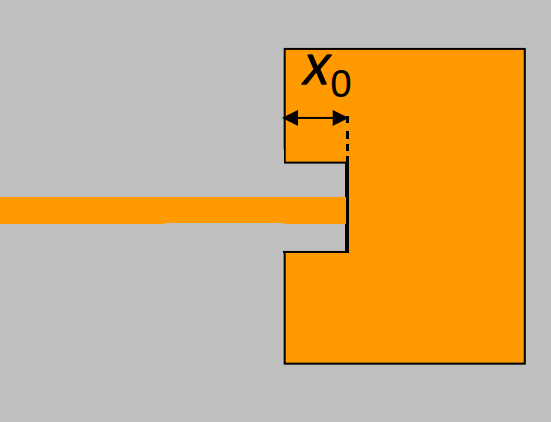
\includegraphics[width=0.4\linewidth]{img/img3}
		\caption{patch antenna with the two slot of lenght $x_0$ in order to have the feeding line matched}
		\label{fig:img3}
	\end{figure}
	\newpage
	\section{DESIGN OF THE PATCH ANTENNA}
	\subsection{Substrate and ground plane size}
	As previously stated, the patch antenna will be mounted on an FR4 material substrate, with a ground plane situated behind it. The initial step is to calculate the dimensions of the board using the following formula:
	\begin{equation}
		W_s=\frac{c}{f_0 \sqrt{\varepsilon_r}}
		\label{Ws}
	\end{equation}
	As can be seen, we need to know the value of $\varepsilon_r$, which is provided in the initial specifications and is equal to:
	\begin{equation}
		\varepsilon_r = 4.1 \cdot (3/f[\text{GHz}])^{0.025}
		\label{epsilon_r}
	\end{equation}
	By substituting with our value of frequency in \eqref{epsilon_r} we obtain: \[\varepsilon_r = 4.1 \cdot (3/2.6[\text{GHz}])^{0.025}=4.11\] 
	so we can now substitute this value in the formula of $W_s$ \eqref{Ws}, but since we are gonna use a square board it will be: \[W_s=L_s=\frac{c}{f_0 \sqrt{\varepsilon_r}}=\frac{3 \cdot 10^8}{2.6 \cdot 10^9\sqrt{4.11}}=0,056882559 m \simeq 56.9\ mm \]
So, now we have the dimensions of the ground plane.
\subsection{Patch size}
In regard to the dimensions of the patch antenna, the width $W_p$ will be calculated using the designated formula \eqref{Wp}, so: 
\[W_p=\frac{3 \cdot 10^8}{2 \cdot 2.6 \cdot 10^9}\sqrt{\frac{2}{4.11+1}}=0,03607639
 \simeq 36.1 \ mm\]
For the length $L_p$, the formula \eqref{Lp} will be employed, with consideration for fringing effects, so first of all we have to determine the value of $\Delta L$, but before doing that we have to calculate the value of $\varepsilon_{eff}$ using the equation \eqref{Epsilon_eff}:
\[\varepsilon_\text{eff} \simeq \frac{4.11 + 1}{2} + \frac{4.11 - 1}{2} \frac{1}{\sqrt{1 + 12 \frac{1.6 \cdot 10^{-3}}{36.1 \cdot 10^{-3}}}}=3,811381 \simeq 3,81\]
so we can now calculate the value of $\Delta L$, by put all the value in the formula \eqref{DeltaL}:
\[	\Delta L \simeq 1.6 \cdot 10^{-3} \cdot 0.412 \frac{\left( 3.81 + 0.3 \right) \left( \frac{36.1 \cdot 10^{-3}}{1.6\cdot 10^{-3}} + 0.264 \right)}{\left( 3.81 - 0.258 \right) \left( \frac{36.1\cdot 10^{-3}}{1.6 \cdot 10^{-3}} + 0.8 \right)} = 0,00074509
\ m \simeq 0.745 \ mm
\]

so, finally we can calculate the value of $L_p$, let's substitute all the value in the equation \eqref{Lp}: 
\[L_p = \frac{3 \cdot 10^8}{2\cdot 2.6 \cdot 10^9 \sqrt{3.81}} - 2\cdot 0.745 \cdot 10^{-3} = 0,02804 \ m \simeq 28.0 \ mm
 \]
  Subsequent to these preliminary calculations, the creation of the substrate may be initiated, with FR4 selected as the material and the various physical values given in the technical specifications. The subsequent steps involve the creation of the ground plane and the design of the patch, with copper chosen as the material for the latter two layers.
 \newpage
 \subsection{Microstrip design}
 After the creation of the substrate and the patch, the microstrip will be created; this should have a characteristic line impedance as close as possible to 50 $\Omega$.
 To achieve this result, we used a macro from CST, the \textit{Impedance calculation} selecting the ‘thick microstrip’ and by putting all our values we start searching for which width of the microstrip would give us an impedance value of 50 $\Omega$, in our case a value of 3.2 mm was chosen as width.
 In the figure below, you can see the use of the macro and note that with the thickness of 3.2 mm, the line impedance is approximately 49.7 ohms.
\begin{figure}[h]
	\centering
	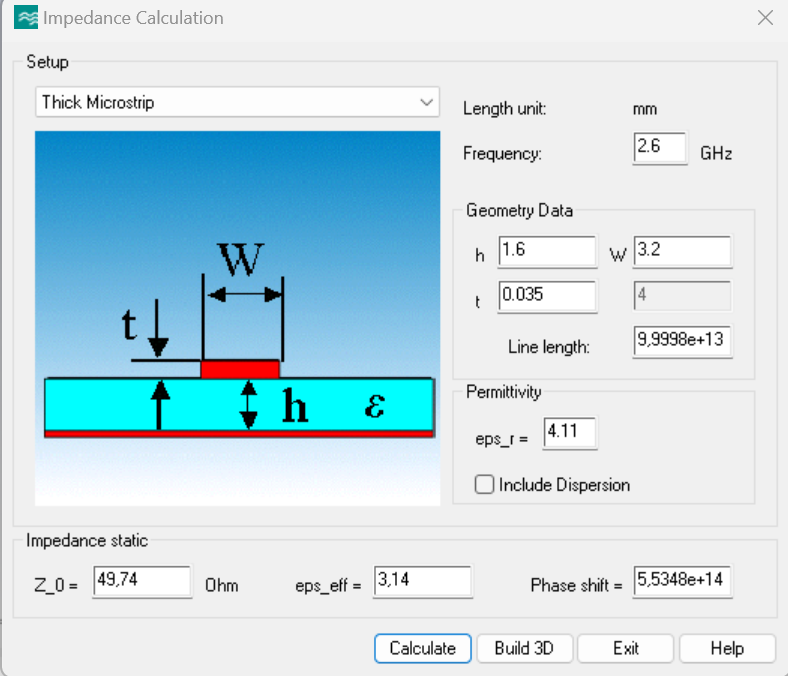
\includegraphics[width=0.30\linewidth]{img/img4}
	\caption{Macro impedance calculation window of CST}
	\label{fig:img4}
\end{figure}

 \subsubsection{Slots design and impedance matching}
 After an initial simulation (the discussion of the results is deferred to the next section), it was necessary to introduce slots on the microstrip in order to improve antenna performance. This intervention made it possible to electrically extend the length of the microstrip, feeding the patch more internally and increasing the impedance seen at the patch input.\\
 In order to find how deep this slot must be, equation \eqref{R_i(x0)} was used by isolating $x_0$, obtaining: 
 \begin{equation}
 	x_0 = \frac{L}{\pi} \arccos\left(\sqrt{2G_1 R_i(x_0)}\right)
 	\label{x0}
 \end{equation}
 where, by substituting the value in \eqref{G_1} we have:
 \[
 G_1=\frac{W}{120 \cdot 115.38 \cdot 10^{-3}
  }\left[ 1-\frac{1}{24}(\frac{2 \pi 1.6\cdot 10^{-3}}{ 115.38 \cdot 10^{-3}})^2\right] = 0.002604694 \simeq 0.0026  
 \]
 so, put the value in \eqref{x0} and obtain: 
 \[
 x_0 = \frac{14.4 \cdot 10^{-3}}{\pi} \arccos\left(\sqrt{2 \cdot 0.0026 \cdot  50}\right) =  0.009241228 \simeq 9.2 \ mm
 \]
so, according to calculations, we will need two slots of approximately 9.2 mm in length.
\begin{figure}[h]
	\centering
	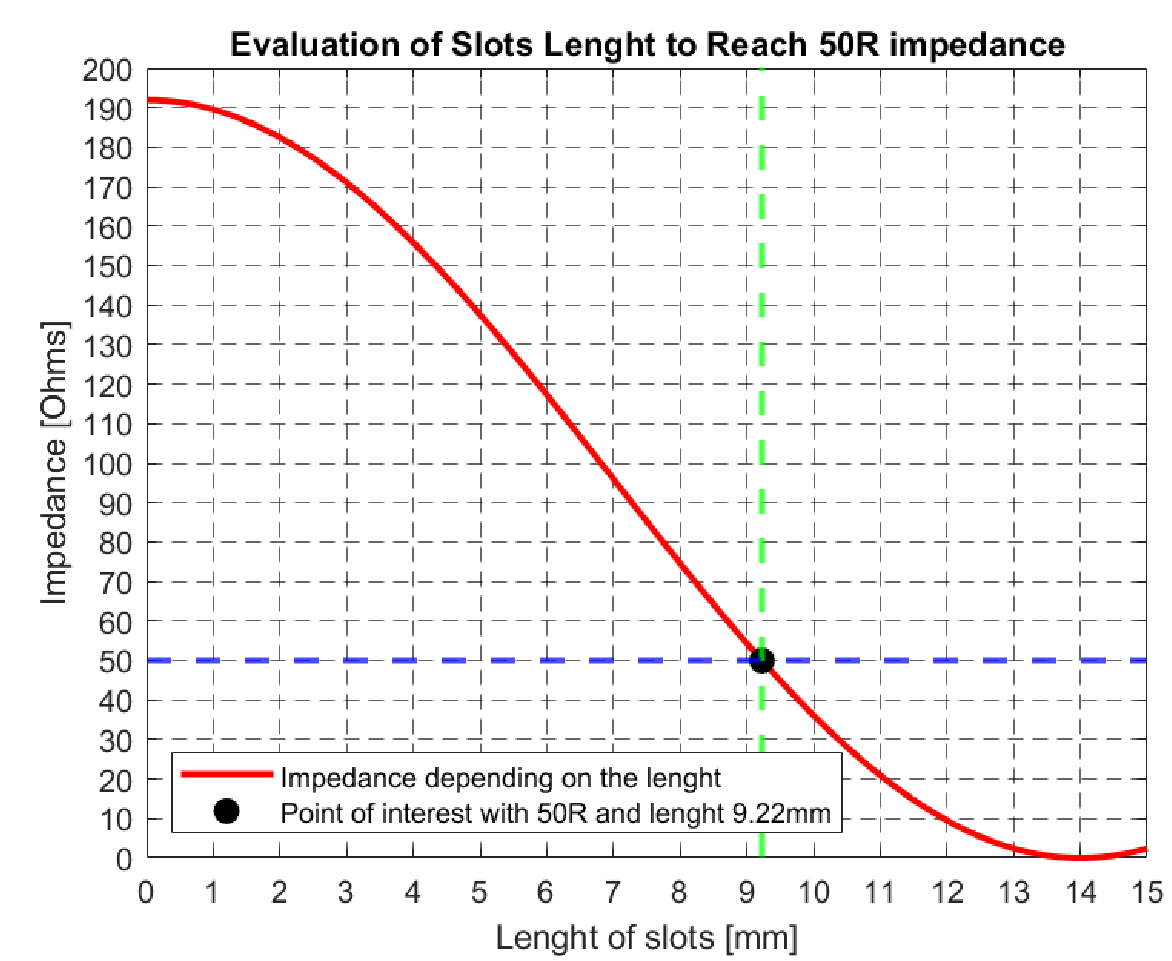
\includegraphics[width=0.42\linewidth]{img/img9}
	\caption{Graph representing the search for the optimum value for slot length, indicating approximately 9.2mm as the length to achieve matching}
	\label{fig:img9}
\end{figure}

\newpage

\subsection{Simulation and tuning}
\subsection{First simulation result}
Following the calculation of the parameters of the patch, the initial simulation was conducted, as illustrated in the subsequent graphs:\\
\begin{figure}[h]
	\centering
	\begin{minipage}{0.4\linewidth}
		\centering
		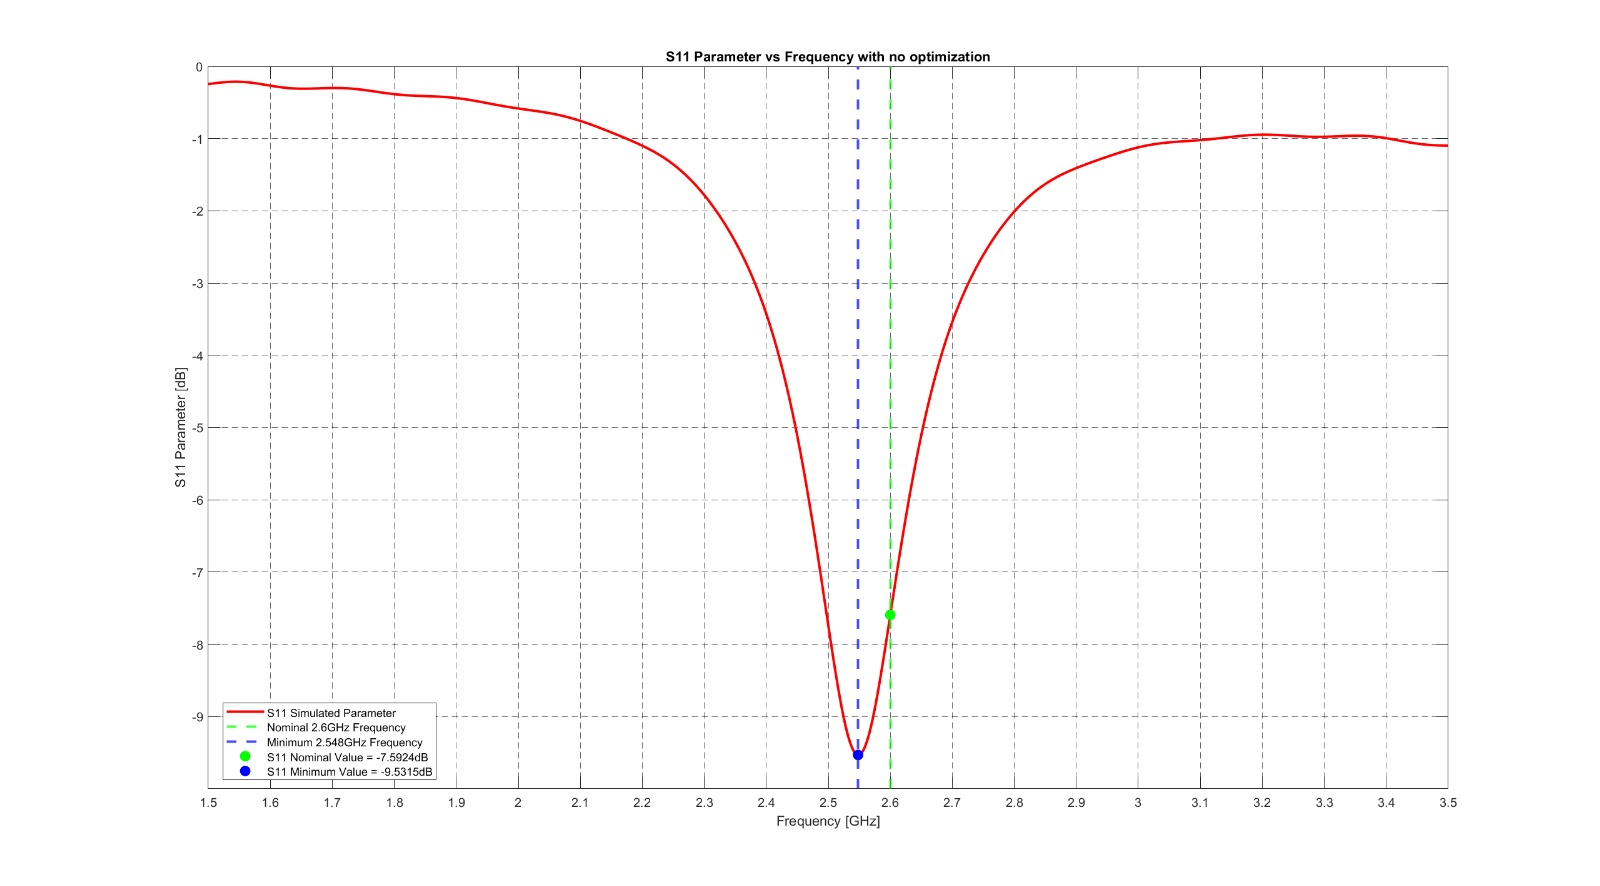
\includegraphics[width=\linewidth]{img/img7}
		\caption{S1,1 graph representing the return loss of the patch antenna during the first simulation without slots}
		\label{GSNOslot}
	\end{minipage}\hspace{0.1\linewidth}
	\begin{minipage}{0.4\linewidth}
		\centering
		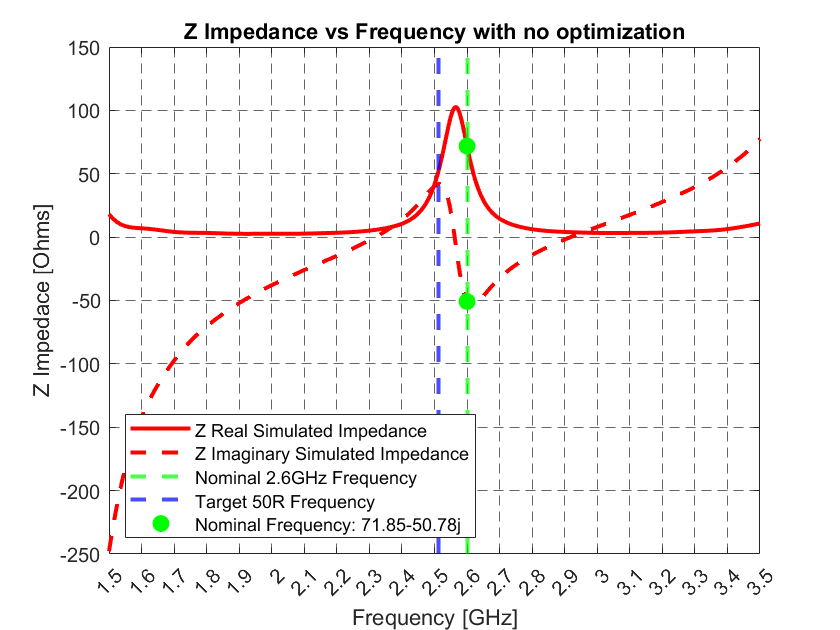
\includegraphics[width=\linewidth]{img/img8}
		\caption{Z graphs representing the values of the real and imaginary part during the first simulation without slots}
		\label{GZNOslot}
	\end{minipage}
\end{figure}

As depicted in Figure \eqref{GSNOslot}, the outcome of the simulation did not meet expectations, exhibiting a peak return loss of approximately -9.5 dB. The figure \eqref{GZNOslot} demonstrates that the microstrip is not entirely matched, exhibiting an impedance of 71.9 $\Omega$ in the real part and a value of approximately 50.8 $\Omega$ in the imaginary part. However, it is observed that the peak frequency falls within the 2.5\% tolerance stipulated by the specifications.
\subsection{Simulation and result with slots}
After this first simulation, the slots were inserted following the measurements from the theoretical calculations. As can be seen in the figures below, the result improved slightly to a peak of -15.0 dB and at 2.6GHz we have the return loss equal to -13.0 dB (figure \eqref{GSslot}) and an impedance value of approximately 32.8 $\Omega$ in the real part and -6.5 $\Omega$  in the imaginary part (figure \eqref{GZslot}).
 \begin{figure}[H]
	\centering
	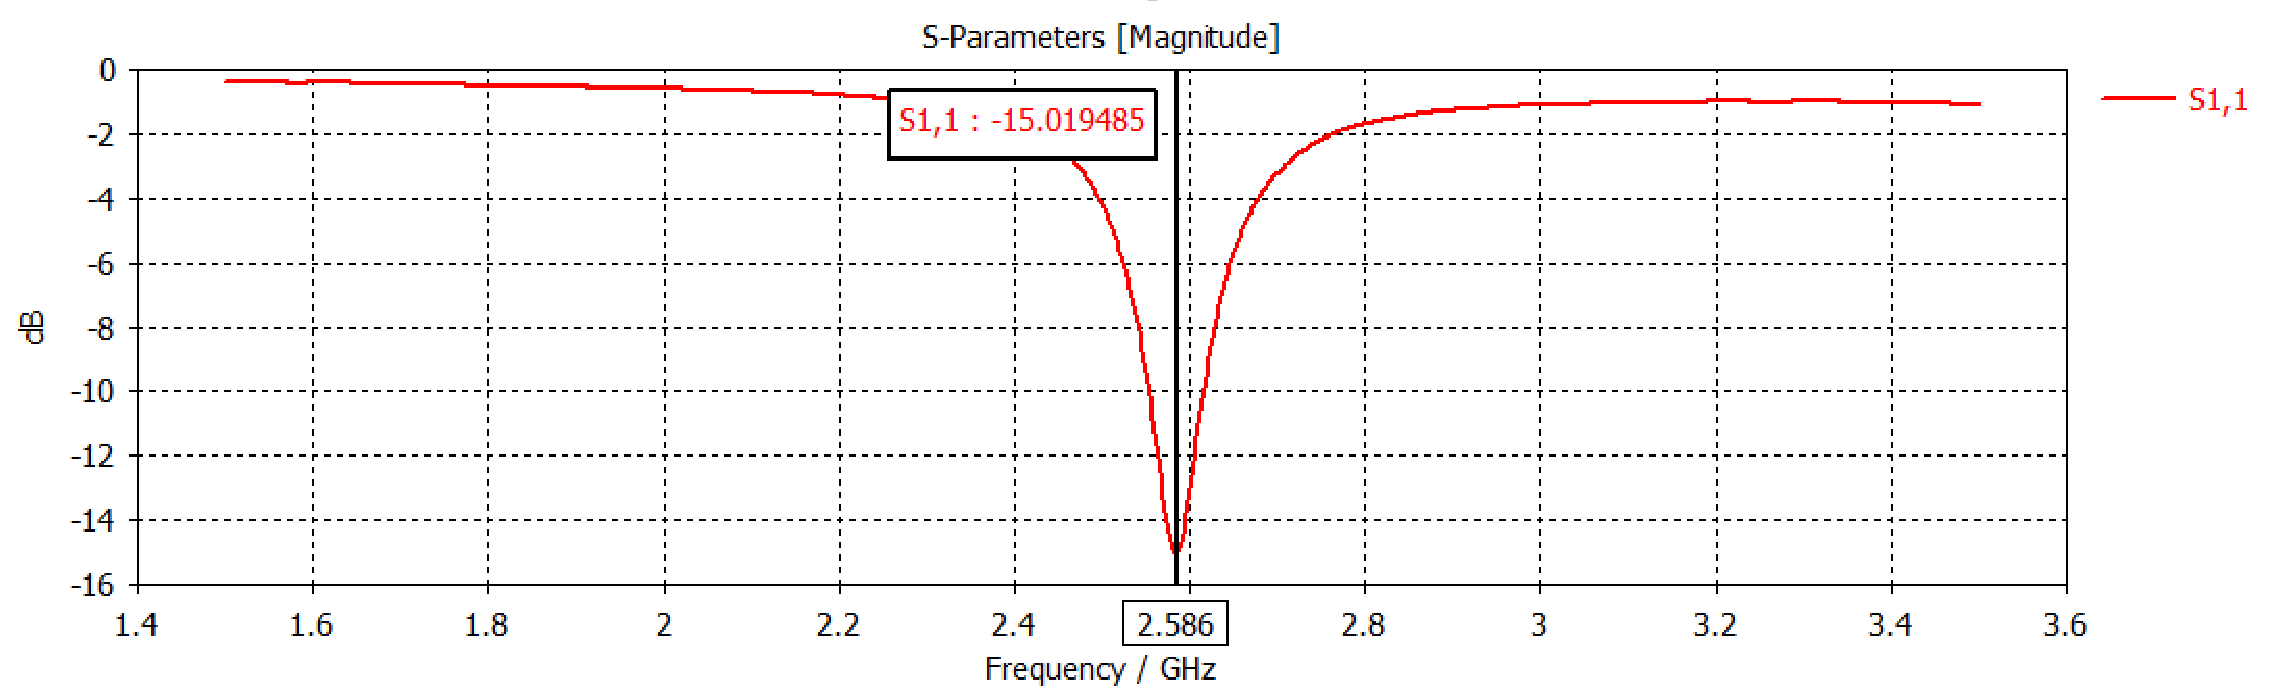
\includegraphics[width=0.85\linewidth]{img/img5}
	\caption{S1,1 graph representing the return loss of the patch antenna with a slots of 9.2mm}
	\label{GSslot}
\end{figure}

\begin{figure}[H]
	\centering
	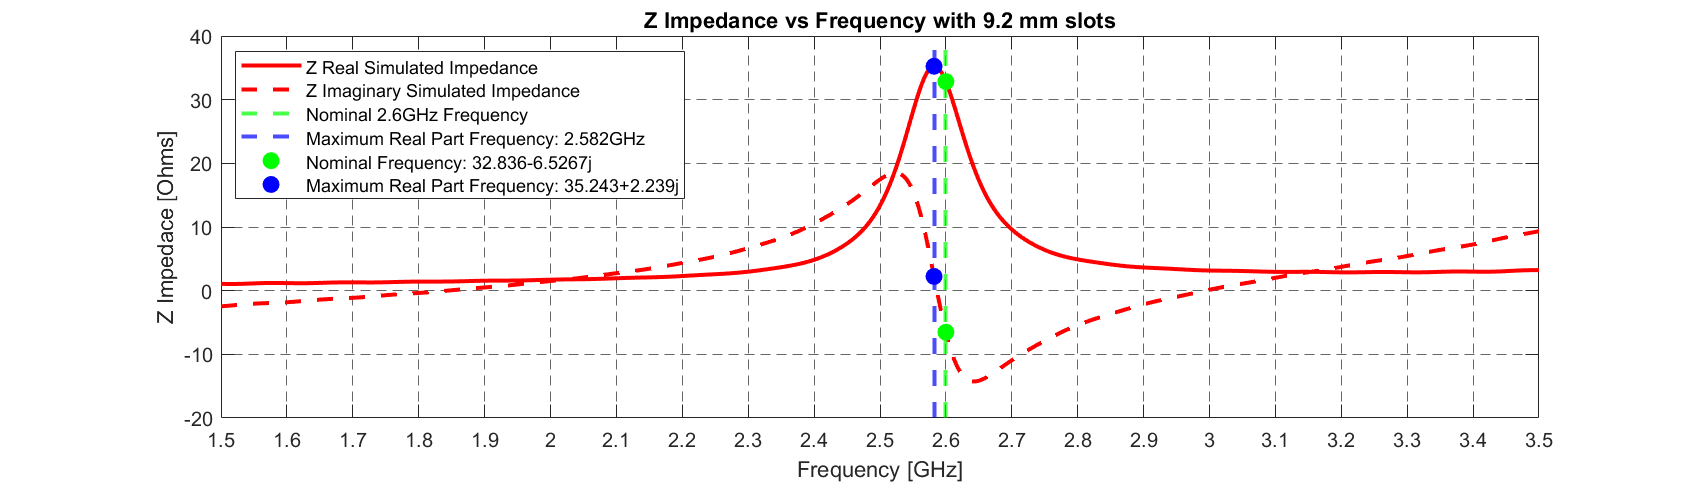
\includegraphics[width=0.85\linewidth]{img/img6}
	\caption{Z graphs representing the impedance of the patch antenna with a slots of 9.2mm}
	\label{GZslot}
\end{figure}
\newpage
 \subsection{Tuning of the patch antenna}
 Starting from the previous results, in order to improve the performance of the antenna, it was necessary to modify certain parameters, in particular the length of the slots, until a value was found that would allow the desired impedance to be achieved and get even closer to the frequency required by the specifications.\\
  In order to assess what was the best possible result, a sweep had to be made, simulating different slot lengths and finding the value that would satisfy the different requirements.\\
  
  
  \begin{figure}[h]
  	\centering
  	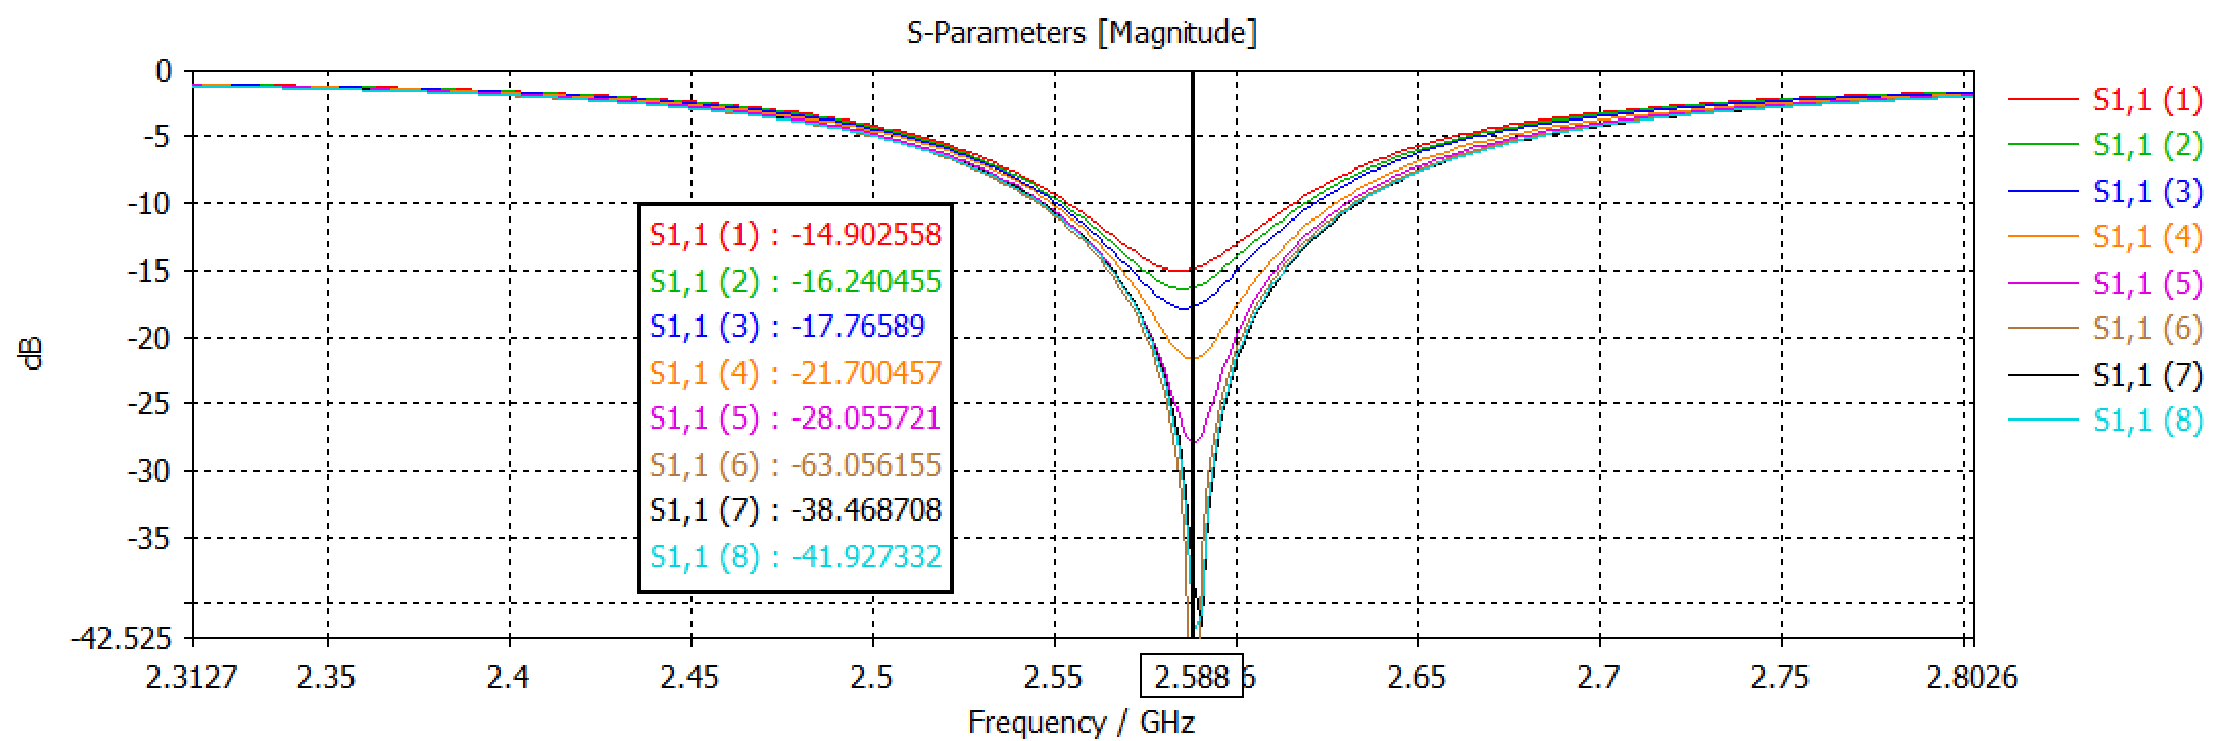
\includegraphics[width=1.0\linewidth]{img/img10}
  	\caption{Graph representing the returning loss of all different values of the slots tested}
  	\label{GSsweep}
  \end{figure}
  As can be seen from the image above, as the slot values were reduced, the peak of the return loss grew and grew until it reached its maximum value, which corresponds to the brown graph, corresponding to a slot length of 7.6 mm.\\
  With this choice, the design of the patch antenna is completed, below is reported the table \eqref{tab:patchDimensions} containing the patch dimensions with a reference image \eqref{RefPatch}.\\

\begin{figure}[H]
	\centering
	\begin{minipage}{0.45\linewidth}
		\centering
		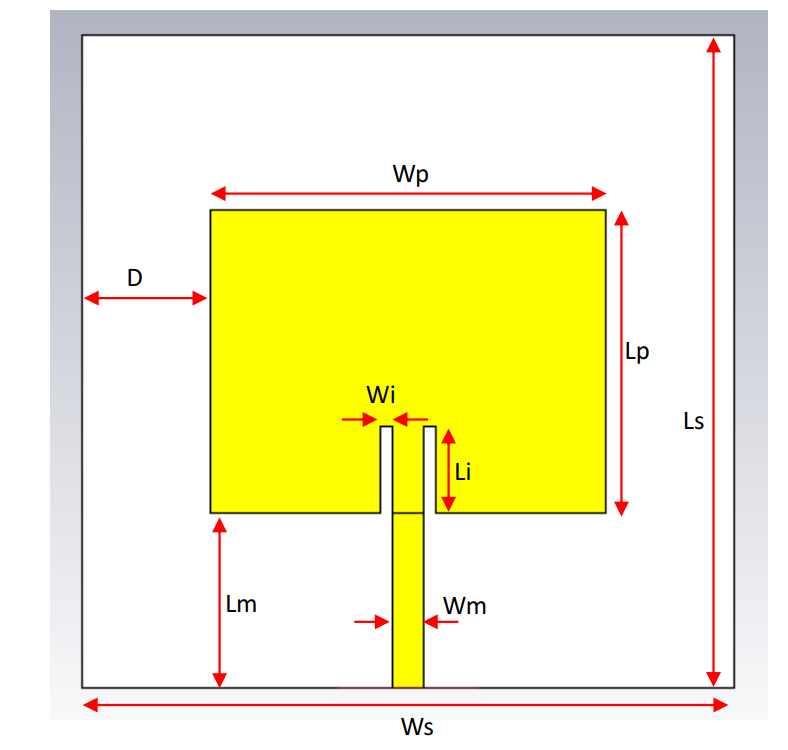
\includegraphics[width=\linewidth]{img/img11}
		\caption{References for the patch antenna dimensions reported in the table alongside}
		\label{RefPatch}
	\end{minipage}\hfill
	\begin{minipage}{0.45\linewidth}
		\centering
		\captionsetup{type=table} % Cambia il tipo di didascalia a 'Table'
		\begin{tabular}{|c|c|}
			\hline
			\textbf{Dimension} & \textbf{Value (mm)} \\
			\hline
			Substrate Width, $W_s$ & 56.9 \\
			Substrate Length, $L_s$ & 56.9 \\
			Microstrip Width, $W_m$ & 3.2 \\
			Microstrip Length, $L_m$ & 14.4 \\
			Distance, $D$ & 10.4 \\
			Slot Width, $W_i$ & 1.0 \\
			Slot Length, $L_i$ & 7.6 \\
			Patch Width, $W_p$ & 36.1 \\
			Patch Length, $L_p$ & 28.0 \\
			\hline
		\end{tabular}
		\caption{Table of patch antenna dimensions}
		\label{tab:patchDimensions}
	\end{minipage}
\end{figure}

\newpage
\section{EXPERIMENTAL: RESULT AND MEASUREMENT}
\subsection{Final simulation}
After the design phase, in which the optimal measurements for the patch antenna were identified, a final simulation was carried out to acquire data that would then be compared with the real measurements.\\
Below are graphs of the three main measurements: return loss, impedance and VSWR.\\

\begin{figure}[h]
	\centering
	\begin{minipage}{0.48\linewidth}
		\centering
		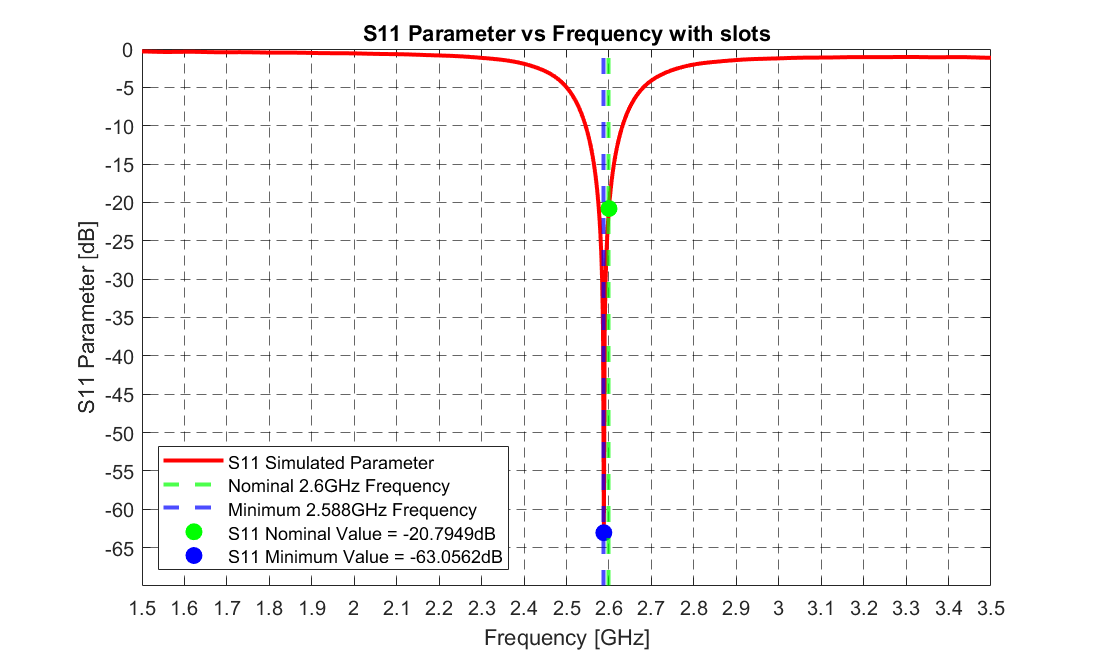
\includegraphics[width=\linewidth]{img/S11_vs_freq_w_slots_small}
		\caption{S11 graph with a slot of 7.6mm}
		\label{S11FIN}
	\end{minipage}
	\hfill
	\begin{minipage}{0.48\linewidth}
		\centering
		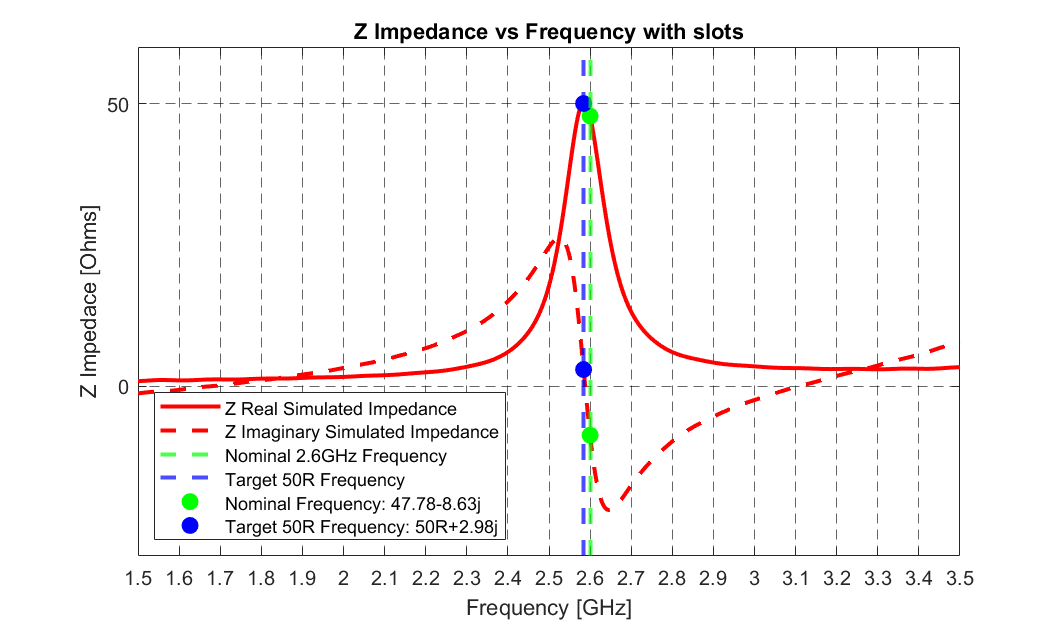
\includegraphics[width=\linewidth]{img/Z_vs_Freq_w_slots_small}
		\caption{Z graph with a slot of 7.6mm}
		\label{ZFIN}
	\end{minipage}
	\\[1em] % Spazio tra le righe
	\begin{minipage}{0.48\linewidth}
		\centering
		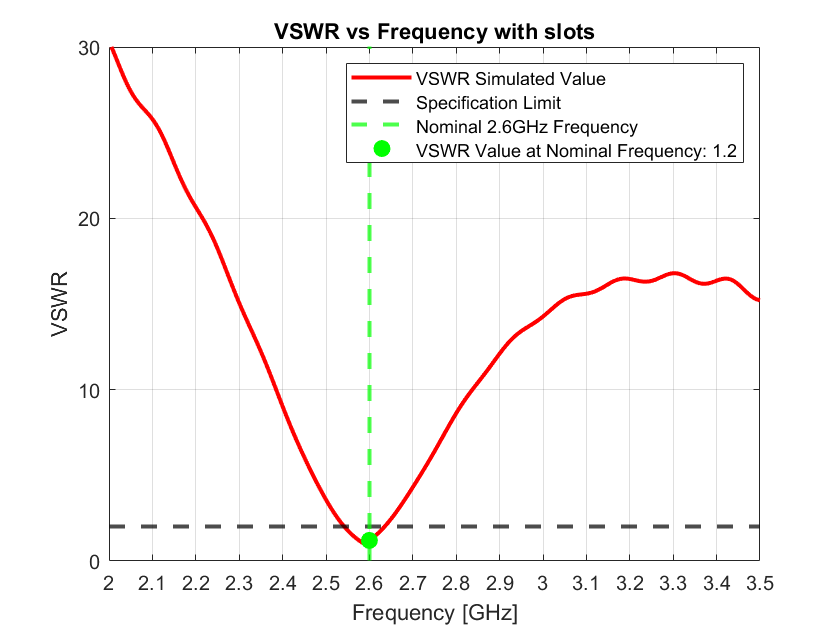
\includegraphics[width=\linewidth]{img/VSWR_with_slot_small}
		\caption{VSWR Graph with a slot of 7.6mm}
		\label{VSWRFIN}
	\end{minipage}
\end{figure}

As we can see from the theoretical values obtained for the patch, we have an excellent result, as we can see in figure \eqref{S11FIN} having a peak value of about -63 dB in the return loss.\\
A second thing we can see is the impedance graph \eqref{ZFIN} where, at the resonance frequency of our antenna, we have an impedance with a real part of about 50 $\Omega$ while the imaginary part is 2.98 $\Omega$, so is a negligible number.

Another graph that can be appreciated is that of the VSWR, which is the ratio measuring the efficiency of impedance matching between the antenna and the transmission line; when this parameter has a value of 1, it indicates perfect matching and minimal reflections. As we can see in the picture \eqref{VSWRFIN}, in this case at the resonance frequency of our antenna the VSWR is equal to 1.2, which means a very good matching that largely respects that required by the specifications. 
The only thing is that in the simulation, the resonance frequency is not quite 2.6 GHz, but a value close enough that still allows to remain well within the required range.
\subsection{Simulation with dummy car}
Another type of simulation performed was using a 3D model of a vehicle to simulate the operation of the patch antenna.\\
For this simulation, the patch was placed at the front of the car, obtaining the result shown in the next page: 
\begin{figure}[H]
	\centering
	\begin{minipage}{0.41\linewidth}
		\centering
		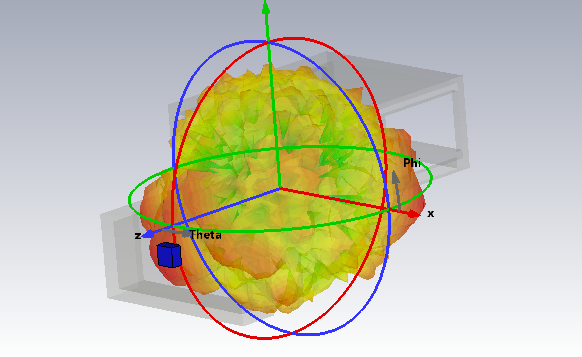
\includegraphics[width=\linewidth]{img/3D_farfield_front_car}
		\caption{far-field 3D plot of the patch antenna with dummy car }
		\label{3Ddummycar}
	\end{minipage}\hspace{0.1\linewidth}
	\begin{minipage}{0.40\linewidth}
		\centering
		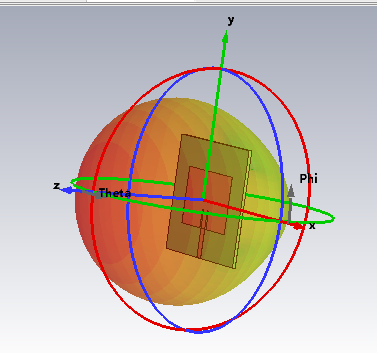
\includegraphics[width=\linewidth]{img/3d_farfield_patchsolo}
		\caption{far-field 3D plot of the patch antenna alone}
		\label{3Dpatch}
	\end{minipage}
\end{figure}


Above, we have in figure \eqref{3Ddummycar} the plot of the far field of our patch integrated in the front of the machine, while in figure \eqref{3Dpatch} we have the same plot but of the patch antenna alone, as can be seen from the analysis of these far-field radiation patterns reveals significant differences between the two radiation patterns.\\
When placed in front of the vehicle, the radiation pattern becomes distorted, showing asymmetry, irregularities and additional side lobes. These distortions can be caused by several factors, for example: reflections, diffraction caused by the metal surfaces and edges of the vehicle redistribute the electromagnetic energy, interfering with the main lobe and creating unwanted secondary lobes, or perhaps the vehicle effectively extends the ground plane of the antenna, changing its impedance and radiation modes. 



\subsection{Real measurements}
Once the desing was finished, the patch antenna was sent into production, the finished result is the one in the picture below:
\begin{figure}[h]
	\centering
	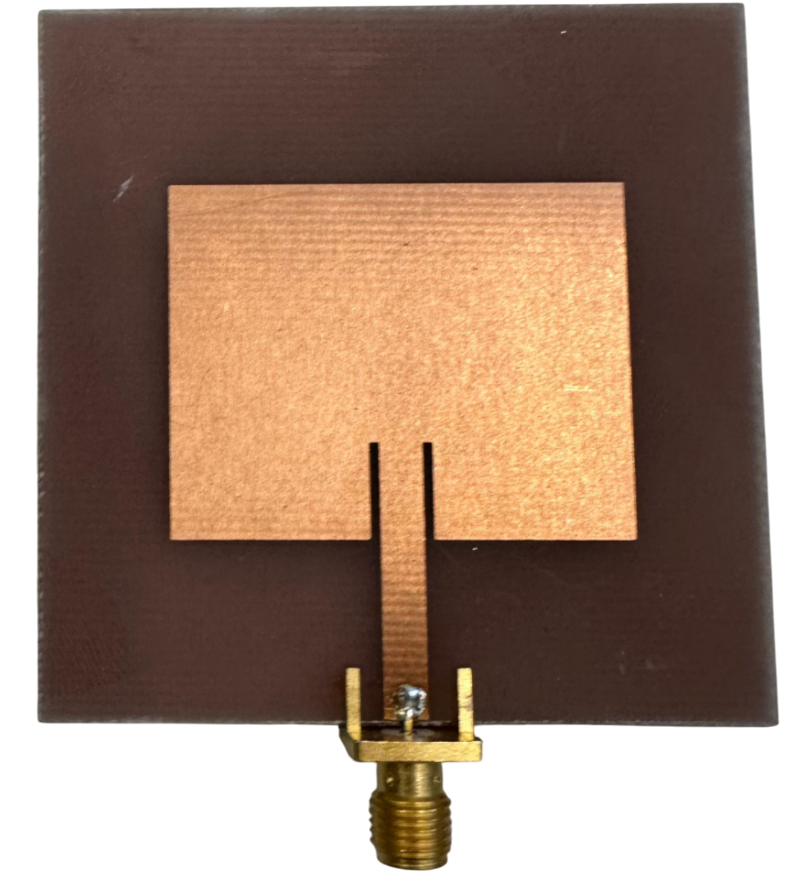
\includegraphics[width=0.35\linewidth]{img/img12}
	\caption{Real patch antenna produced according to the dimensions reported in the table \eqref{tab:patchDimensions}}
	\label{realpatch}
\end{figure}


After obtaining the physical patch, measurements were carried out in the laboratory using a Horn antenna, a network analyzer and other supports, including a rotating tripod used to measure the radiation pattern.\\
The measurement station is shown in the figure \eqref{MEASSTATION} in the next page:
\begin{figure}[H]
	\centering
	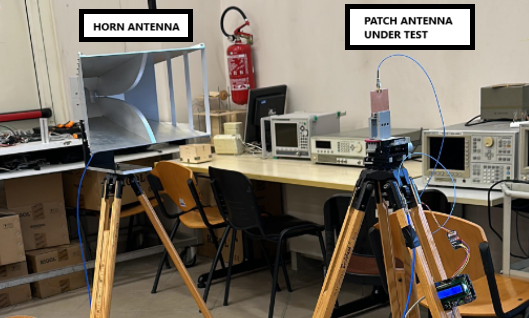
\includegraphics[width=0.5\linewidth]{img/img13}
	\caption{Measurement station composed by: horn antenna, patch antenna and a network analyzer (not present in the image)}
	\label{MEASSTATION}
\end{figure}

The horn and the patch antennas are connected to a network analyzer, which measures the electrical performances of radio-frequency components, such as S11 to evaluate signal behavior and impedance matching.\\
The horn antenna serves as a stationary receiver, leveraging its high bandwidth to detect the electromagnetic field radiated by the patch antenna during measurements.\\
\subsubsection{Measurement of S11 and matching impedance}
As a first measurement, after the proper calibration, the S11 of the antenna was measured, obtaining the real value of the return loss, from which the matching impedance can be determined.\\
The following graphs \eqref{s11vsfreqrealcropped} and \eqref{zvsfreqrealdatacropped} represent the real value measured of the antenna: 
\begin{figure}[H]
	\centering
	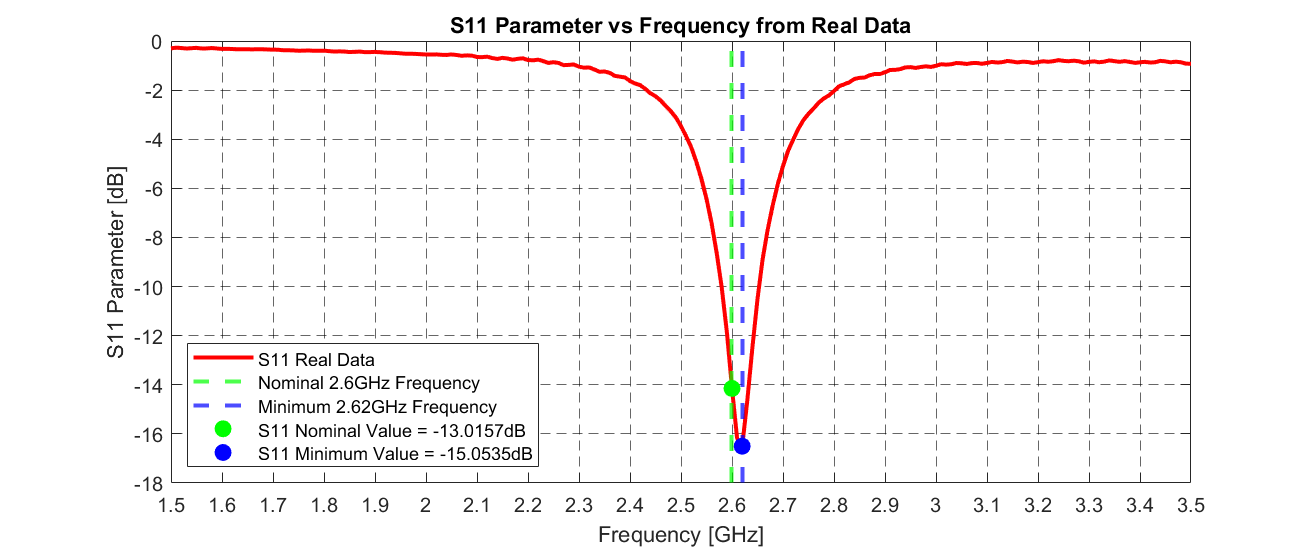
\includegraphics[width=0.7\linewidth]{img/S11_vs_freq_real_cropped}
	\caption{S11 real measurement of the patch antenna}
	\label{s11vsfreqrealcropped}
\end{figure}

\begin{figure}[h]
	\centering
	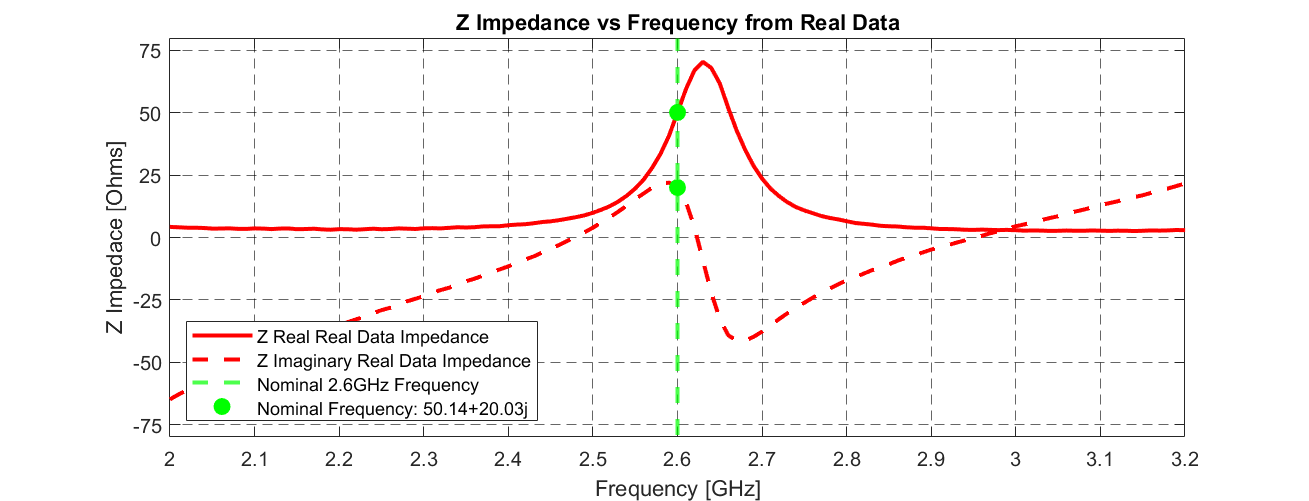
\includegraphics[width=0.7\linewidth]{img/Z_vs_freq_real_data_cropped}
	\caption{Impedance values derived from real measurement }
	\label{zvsfreqrealdatacropped}
\end{figure}

From the graphs above, it can be seen that, compared to the simulated version, the peak is centered at 2.62 GHz instead of 2.58 GHz, with a value around -15 dB.\\
This result, while acceptable, does not reach the excellence shown in the simulations. With regards to the impedance matching, it can be observed that at a frequency of 2.6 GHz, the real value is approximately 50 $\Omega$, while the imaginary part is around 20 $\Omega$. This indicates that the impedance matching is not optimal, as the imaginary component signifies a residual reactance that has the potential to influence the antenna's overall performance. Such a scenario could be attributed to manufacturing imperfections, mismatches, or parasitic effects that were not anticipated during the simulation process. 
\subsubsection{Radiation pattern measurement}
After the first type of measurement, radiation pattern measurements were carried out. For this purpose, the rotating tripod was used: the measurement was carried out and, with each measurement, the patch antenna was rotated by 2°; the procedure was then repeated by rotating the patch antenna by 90°, so that both the vertical (E-plane) and horizontal (H-plane) planes were evaluated.
The measurements produced the following results: 
\begin{figure}[H]
	\centering
	\begin{minipage}{0.41\linewidth}
		\centering
		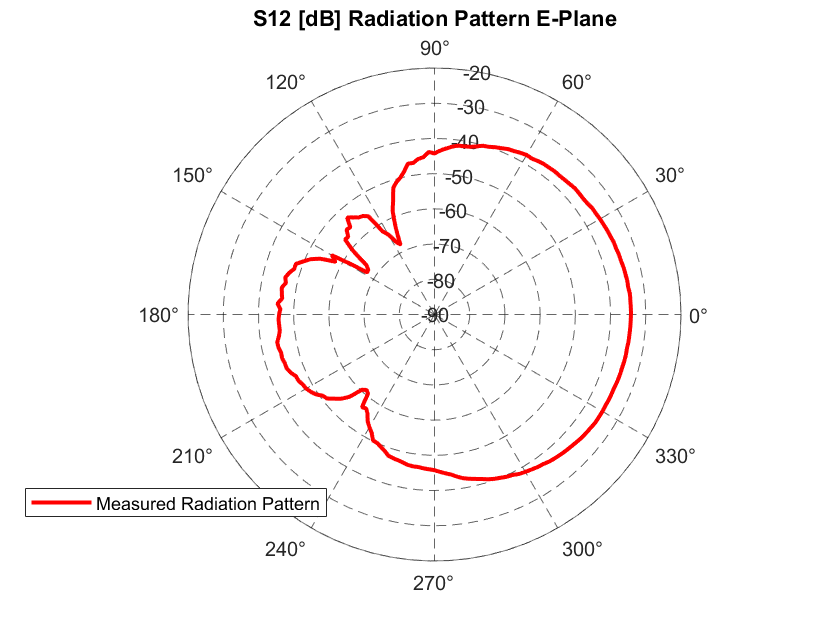
\includegraphics[width=\linewidth]{img/S12_vs_angle_rad_pattern_no_comp_eplane_small}
		\caption{Radiation pattern of the vertical plane}
		\label{Epln-solo}
	\end{minipage}\hspace{0.1\linewidth}
	\begin{minipage}{0.42\linewidth}
		\centering
		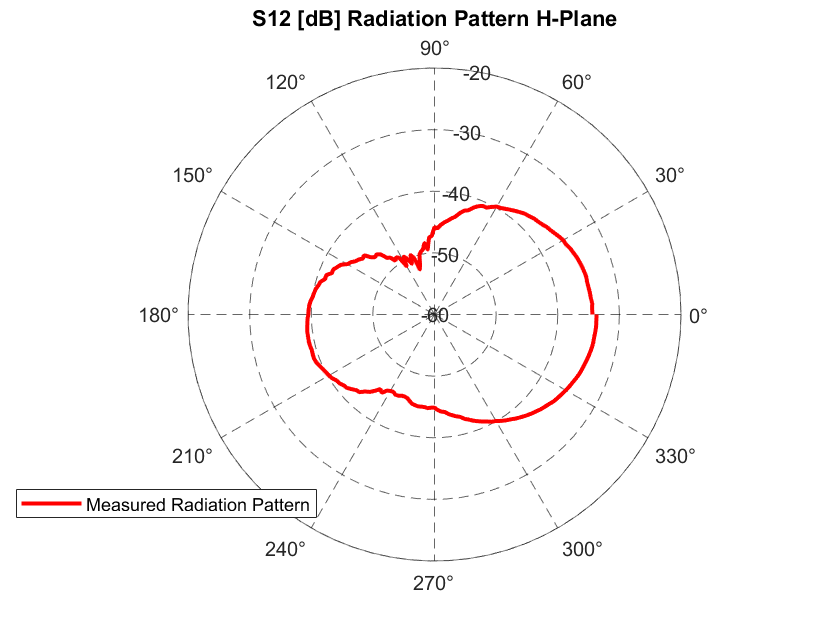
\includegraphics[width=\linewidth]{img/S12_vs_angle_rad_pattern_no_comp_hplane_small}
		\caption{Radiation pattern of the horizontal plane}
		\label{Hpln-solo}
	\end{minipage}
\end{figure}
\section{RESULT COMPARISON}
Below are reported the graphs comparing the measured values with those obtained from simulations:
\begin{figure}[H]
	\centering
	\subfloat[Comparison between the return loss simulated (pink) and measured (red)]{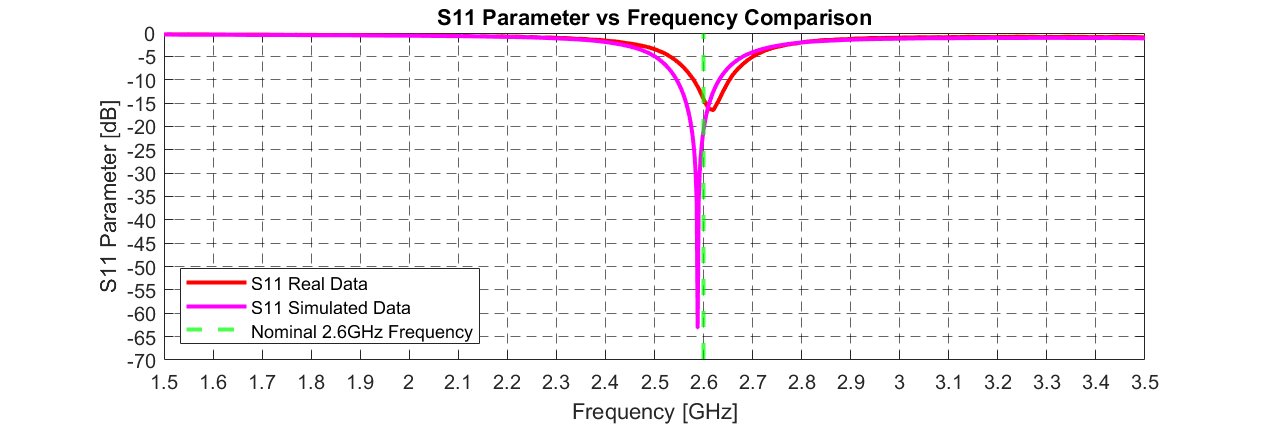
\includegraphics[width=0.45\linewidth]{img/COMPARISON/S11_vs_freq_comparison_real_simulated} \label{fig:s11vsfreqcomparisonrealsimulated}} \hspace{0.5cm}
	\subfloat[Comparison between simulated impedance (blue) and measured (red)]{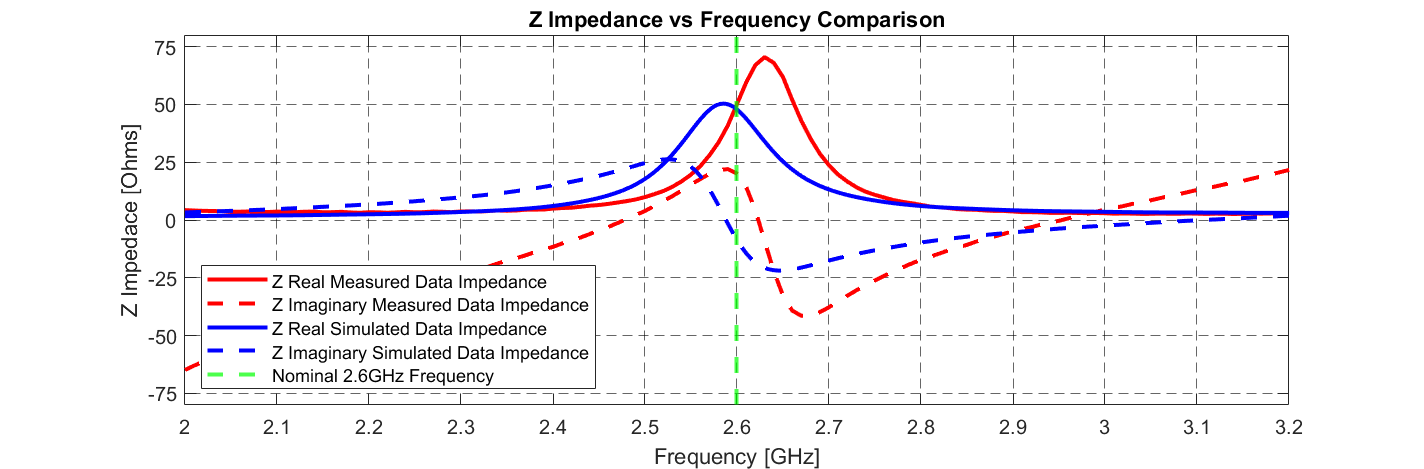
\includegraphics[width=0.45\linewidth]{img/COMPARISON/Z_vs_freq_comparison_cropped} \label{fig:zvsfreqcomparisoncropped}} \\
	\subfloat[Comparison between the vertical plane simulated (blue) and meausred (red)]{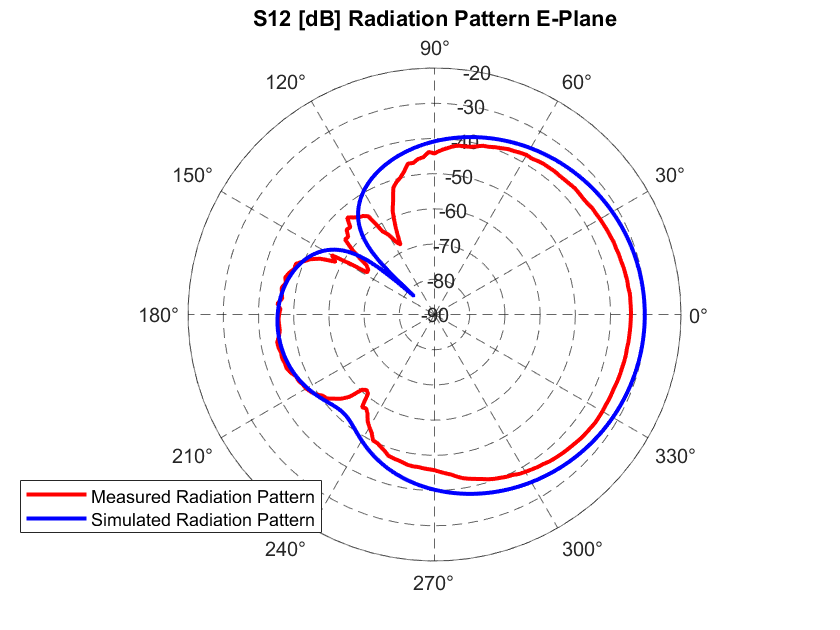
\includegraphics[width=0.40\linewidth]{img/COMPARISON/S12_vs_angle_rad_pattern_eplane_small} \label{fig:s12vsangleradpatterneplanesmall}} \hspace{0.5cm}
	\subfloat[Comparison between the horizontal plane simulated (blue) and meausred (red)]{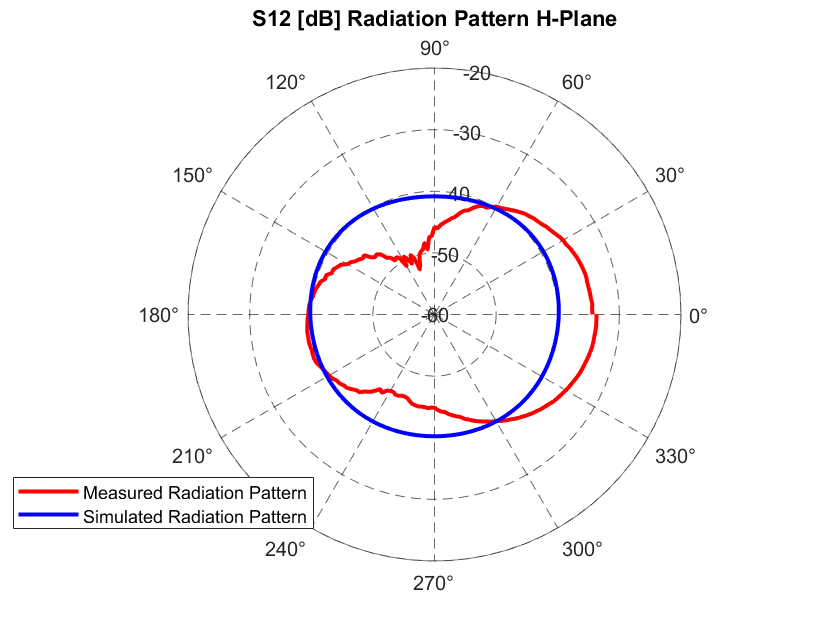
\includegraphics[width=0.40\linewidth]{img/COMPARISON/S12_vs_angle_rad_pattern_hplane_small} \label{fig:s12vsangleradpatterneplanesmall2}}
	
	\label{fig:2x2images}
\end{figure}
As can be seen from the superimposed graphs, for what concern the return loss and impedance, as mentioned earlier, there was a reduction in the S11 peak from -63dB to -15dB and an increase in the imaginary part of the impedance from about 2 $\Omega$ to about 20 $\Omega$.
The comparison between the measured and simulated radiation patterns shows notable differences for the E-plane and H-plane. In the E-plane (vertical), the simulated pattern closely matches the measured one, showing good accuracy in predicting the behavior of the antenna. Minor discrepancies are observed in the side lobes and parts of the main lobe, where the simulated pattern appears smoother than the measured data.
In the H-plane (horizontal) the discrepancies are more pronounced. The measured pattern shows more irregularities, with stronger and less symmetrical side lobes compared to the simulation, possible causes of all these differences, both in the parameters and in the radiation patterns, can be: tolerances in the board manufacture, irregularities in the materials used, coupling with adjacent objects or reflections during the measurement phase.\\
To solve these problems and improve antenna performance, possible solutions are: 
\begin{itemize}
	\item \textbf{Vary the patch dimensions}: Adjusting not only the slots length but also the slots width or the overall patch size could help fine-tune the resonant frequency and improve impedance matching
	\item \textbf{Optimize the test environment}: Perform measurements in a more open environment to reduce the risk of interference, or ideally, in an Anechoic chamber to eliminate reflections and ensure more accurate radiation pattern measurements
\end{itemize}
\subsection{Summary of results}
The following tables summarize the results of the patch antenna analysis. The first table (table \eqref{tabmeasure}) compares the analytical values with those obtained during the simulation, aimed at optimizing the antenna design. The second table (table \eqref{tabS11}) highlights the differences between the final simulated values and the measured results:
\begin{center}
	 \captionsetup{type=table} % Cambia il tipo di didascalia a 'Table'
	\begin{tabular}{|c|c|c|}
		\hline
		\textbf{Dimension} & \textbf{Analytical Value (mm)} & \textbf{Final Value (mm)} \\
		\hline
		Substrate Width, $W_s$ & 56.9 & 56.9\\
		\hline
		Substrate Length, $L_s$ & 56.9 & 56.9\\
		\hline
		Microstrip Width, $W_m$ & 3.2 & 3.2\\
		\hline
		Microstrip Length, $L_m$ & 14.4& 14.4\\
		\hline
		Distance, $D$ & 10.4 & 10.4\\
		\hline
		Slot Width, $W_i$ & 1.0 & 1.0\\
		\hline
		Slot Length, $L_i$ & 9.2 & 7.6\\
		\hline
		Patch Width, $W_p$ & 36.1 & 36.1\\
		\hline
		Patch Length, $L_p$ & 28.0 & 28.0\\
		\hline
	\end{tabular}
	\caption{Table comparing the analytic dimensions of the patch antenna and the final ones}
	\label{tabmeasure}
\end{center}
\begin{center}
	\captionsetup{type=table} % Cambia il tipo di didascalia a 'Table'
	\begin{tabular}{|c|c|c|}
		\hline
		\textbf{Parameter} & \textbf{Simulated Value} & \textbf{Measured Value} \\
		\hline
		Resonance Frequency & 2.588 GHz & 2.620 GHz\\
		\hline
		Return Loss & -63.05 dB & -15.05 dB\\
		\hline
		Impedance & $50 + j2.98 \, \Omega$ & $50.14 + j20.03 \, \Omega$\\
			\hline
	\end{tabular}
	\caption{Table comparing the simulated values and the real measured ones}
	\label{tabS11}
\end{center}
\section{CONCLUSIONS}
The aim of the laboratory experience was to create a patch antenna that met certain requirements, which allowed us to put some theoretical concepts into practice and gain experience with the CST software and some laboratory instruments, allowing us to make real measurements.\\ Unfortunately, some real results, although within the required specifications, did not match the simulation results, which allowed us to think about possible causes and future implementations or solutions to further improve our patch antenna.
	%FINE DOCUMENTO
\end{document}